%From https://egu2018.eu/PICO_how-to_guide_to_PICO.pdf
%Abstracted and templated by Brian Ballsun-Stanton, Macquarie University.
%original template by https://github.com/snowtechblog/pico-latex-presentation by Anselm Köhler

%Pico Presentation Ratio: 169
\documentclass[unknownkeysallowed,usepdftitle=false, aspectratio=169,parskip=full]{beamer}
% unknownkeysallowed is needed for mac and the newer latex version -> is more picky than before...
\usetheme[headheight=1cm,footheight=2cm]{boxes}
%\usetheme{default}

\usepackage{multicol}

\usepackage{default}
\usepackage{graphicx}
%example pictures created via: http://lorempixel.com/1200/800/cats/Figure2/. Credit to http://lorempixel.com/images.php

\usepackage{epsfig}
\usepackage{siunitx}
\usepackage{color}
\usepackage{ifthen}
%usepackage{ragged2e}

\usepackage[T1]{fontenc}
\usepackage[utf8]{inputenc}
%https://tex.stackexchange.com/a/203804/5483

\usepackage[activate={true,nocompatibility},final,tracking=true,kerning=true,spacing=true,factor=1100,stretch=10,shrink=10]{microtype} % http://www.khirevich.com/latex/microtype/
\microtypecontext{spacing=nonfrench}

\usepackage[UKenglish]{babel} %https://tex.stackexchange.com/a/27743 
\usepackage[pangram]{blindtext} % https://tex.stackexchange.com/a/48411

%\usepackage{parskip} % from https://tex.stackexchange.com/q/11622
%\setlength{\parskip}{12pt} 

%\setparsizes{\parindent}{12pt}{\parfillskip}

%\usepackage{etoolbox} % as per https://tex.stackexchange.com/a/24331
%\appto\chapterheadendvskip{\vspace{-1\parskip}}
%\setparsizes{\parindent}{50pt plus 20pt minus 30pt}{\parfillskip}

\setbeamertemplate{navigation symbols}{}%remove navigation symbols
\setbeamersize{text margin left=1cm,text margin right=1cm}

% some colors
\definecolor{grau}{gray}{.5}
\definecolor{slfcolor}{rgb}{0,0.6274,0.8353}
\definecolor{wslcolor}{rgb}{0,0.4,0.4}

% setup links
\hypersetup{%
	%linkbordercolor=green,%
	colorlinks=false,%
	pdfborderstyle={/S/U/W 0},%
	%pdfpagemode=FullScreen,%
	pdfstartpage=4%
	}

% setup some fonts
\setbeamerfont{title}{series=\bfseries, size=\small}
\setbeamerfont{author}{size*={5pt}{0pt}}
\setbeamerfont{institute}{size*={3pt}{0pt}}
\setbeamerfont{bodytext}{size=\scriptsize}
	
% Title setup	
\title{Planning for Publication}
\author{Sheriden Goldie (\texttt{sheriden.goldie@hdr.mq.edu.au})}
\institute{Macquarie University, Sydney, NSW
}
% add title in headbox
\setbeamertemplate{headline}
{\leavevmode
\begin{beamercolorbox}[width=1\paperwidth]{head title}
  % LOGO
  \vspace{0.1cm}
  \begin{columns}[t, totalwidth=\textwidth]
  \begin{column}[c]{1.05cm}
    
  \end{column}
  % TITLE
   \begin{column}[c]{10.6cm}
   \centering \usebeamerfont{title} \textcolor{slfcolor}{\inserttitle} \\
   \centering \usebeamerfont{author} \color[rgb]{0,0,0} \insertauthor \\
   \vspace{-0.05cm}
   \centering \usebeamerfont{institute} \insertinstitute
  \end{column}
  % PICTURE
  \begin{column}[c]{1.15cm}
    \hspace{0.005cm}
    
\includegraphics[width=1cm]{Images/MQ_INT_VER_RGB_POS.png}
  \end{column}
  \end{columns}
  {\color{slfcolor}\hrule height 1pt\vspace{0.1cm}}
\end{beamercolorbox}%
}

% setup the navigation in footbox
% first set some button colors
\newcommand{\buttonactive}{\setbeamercolor{button}{bg=wslcolor,fg=white}}
\newcommand{\buttonpassive}{\setbeamercolor{button}{bg=slfcolor,fg=black}}
% now set up that the one active one gets the new color.
\newcommand{\secvariable}{nothing}
% therefore we write before each section (well, everything which should be part of the navi bar)
% the variable \secvariable to any name which is in the next function ...
\newcommand{\mysection}[1]{\renewcommand{\secvariable}{#1}
}
% ... compaired to strings in the following navibar definition ...
\newcommand{\tocbuttoncolor}[1]{%
 \ifthenelse{\equal{\secvariable}{#1}}{%
    \buttonactive}{%
    \buttonpassive}
 }
% ... here we start to set up the navibar. each entry is calling first the function \tocbuttoncolor with the argument which should be tested for beeing active. if active, then change color. afterwards the button is draw. so to change that, you need to change the argument in \toc..color, the first in \hyperlink and before each frames definition... A bit messed up, but works...
\newlength{\buttonspacingfootline}
\setlength{\buttonspacingfootline}{-0.2cm}
\setbeamertemplate{footline}
{\leavevmode
\begin{beamercolorbox}[width=1\paperwidth]{head title}
  {\color{slfcolor}\hrule height 1pt}
  \vspace{0.05cm}
  % set up the buttons in an mbox
  \centering \mbox{
    \tocbuttoncolor{abstract}
    \hyperlink{abstract}{\beamerbutton{2 Minute Madness}}
    \tocbuttoncolor{radar}
    \hspace{\buttonspacingfootline}
      \hyperlink{radar}{\beamerbutton{Section 1}}

    \tocbuttoncolor{line}
    \hspace{\buttonspacingfootline}
      \hyperlink{line}{\beamerbutton{Section 2}}
    \tocbuttoncolor{major}
    \hspace{\buttonspacingfootline}
      \hyperlink{major}{\beamerbutton{Section 3}}
    \tocbuttoncolor{slab}
    \hspace{\buttonspacingfootline}
      \hyperlink{slab}{\beamerbutton{Section 4}}
    
    % this last one should normalLy not be used... it will open the preferences to change the 
    % behaviour of the acrobat reader in fullscreen -> usefull in pico...
    \setbeamercolor{button}{bg=white,fg=black}
    % for presentation
    %\hspace{-0.1cm}\Acrobatmenu{FullScreenPrefs}{\beamerbutton{\#}}
    % for upload
    
     
\Acrobatmenu{FullScreenPrefs}{\vspace{0.3cm}\hspace{0.24cm}\mbox{%
      
\includegraphics[height=0.04\textheight,keepaspectratio]{Images/CCLicense.png}
	  }}
   }
    \vspace{0.05cm}
\end{beamercolorbox}%
}


\begin{document}


%%%%%%%%%%%%%%%%%%%%%%%%%%%%%%%%%%%%%%%%%%%%%%%%%%%%%%%%%%%%%%%%%%%%%%%%%%
\mysection{abstract}
%%%%%%%%%%%%%%%%%%%%%%%%%%%%%%%%%%%%%%%%%%%%%%%%%%%%%%%%%%%%%%%%%%%%%%%%%%
\begin{frame}\label{\secvariable}

\usebeamerfont{bodytext}


\begin{columns}[t]
  %https://tex.stackexchange.com/a/7452/5483
  \begin{column}[c]{0.45\textwidth}

%Original template: https://github.com/snowtechblog/pico-latex-presentation by Anselm Köhler


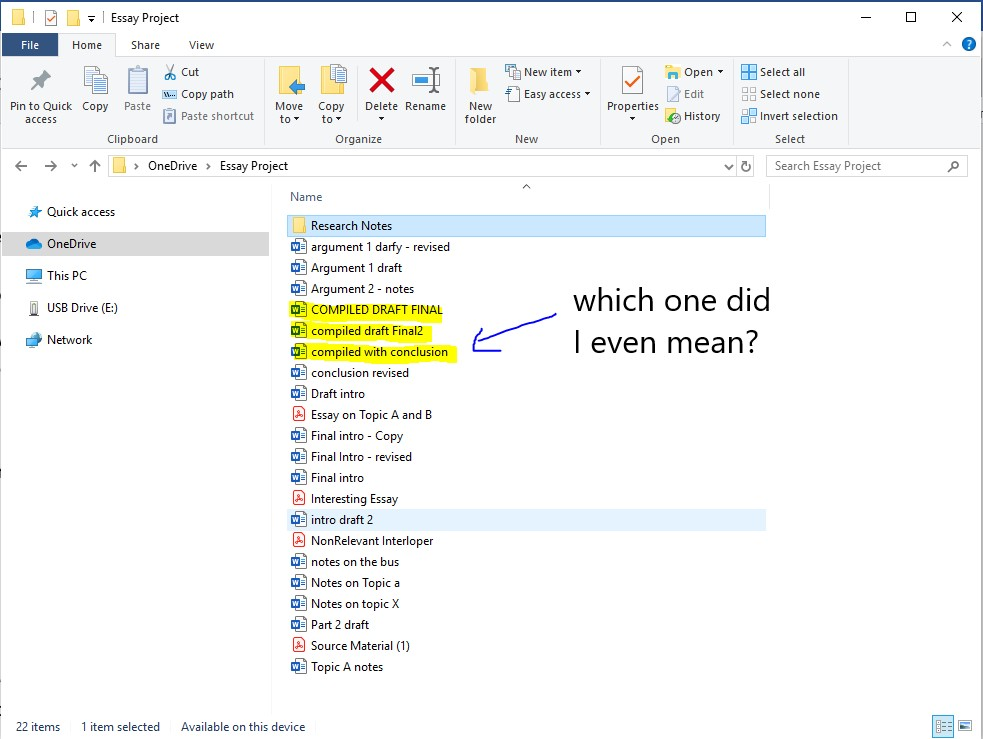
\includegraphics[width=7cm]{Images/MessyFolder.jpg}


 \vspace{12pt}
\end{column}


\begin{column}[c]{0.45\textwidth}

\textbf{Organising a research/creative project is hard.}
\vspace{6pt}

To try and reduce the pain of this:

\includegraphics[width=3cm]{Images/WayArrow.png}


I needed to:
\begin{itemize}
    \item Creating an organisational structure to enable the composition of a large multifaceted project
    \item Streamline the document finalisation process to enable a more timely delivery of finished documents, with less STRESS!
\end{itemize}

\end{column}

\end{columns}


\end{frame}

\begin{frame}\label{\secvariable}
  \begin{multicols*}{3}
  Using Scrivener, my folder full of drafts, notes and redrafts, now looks like this: 
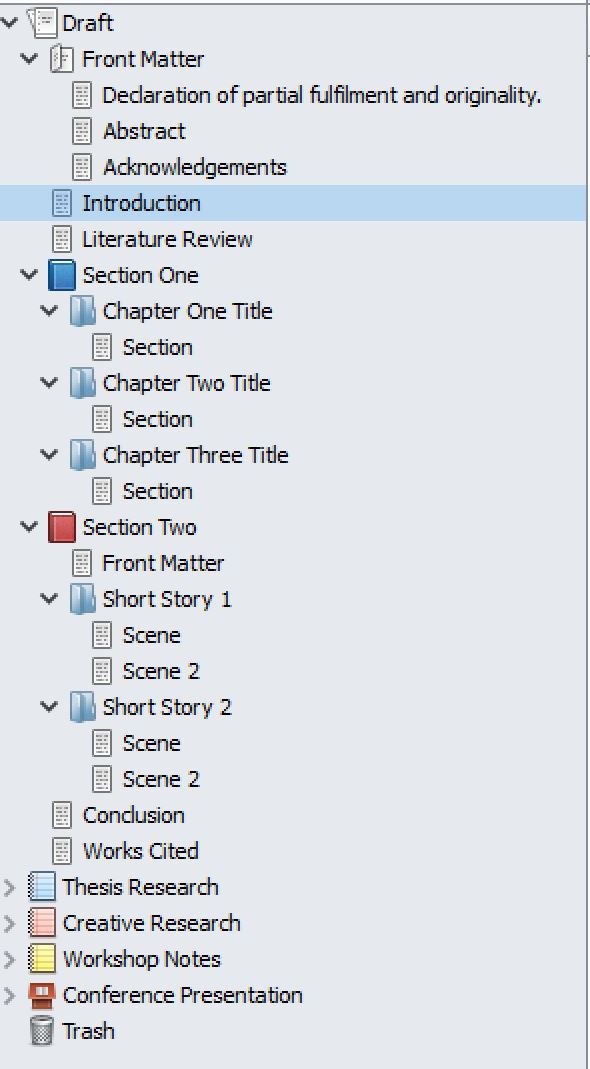
\includegraphics[width=3cm,keepaspectratio]{Images/ScrivFolderStructure.JPG}
\columnbreak %Column break point

      I can now take a document from Scrivener and turn it from this:
   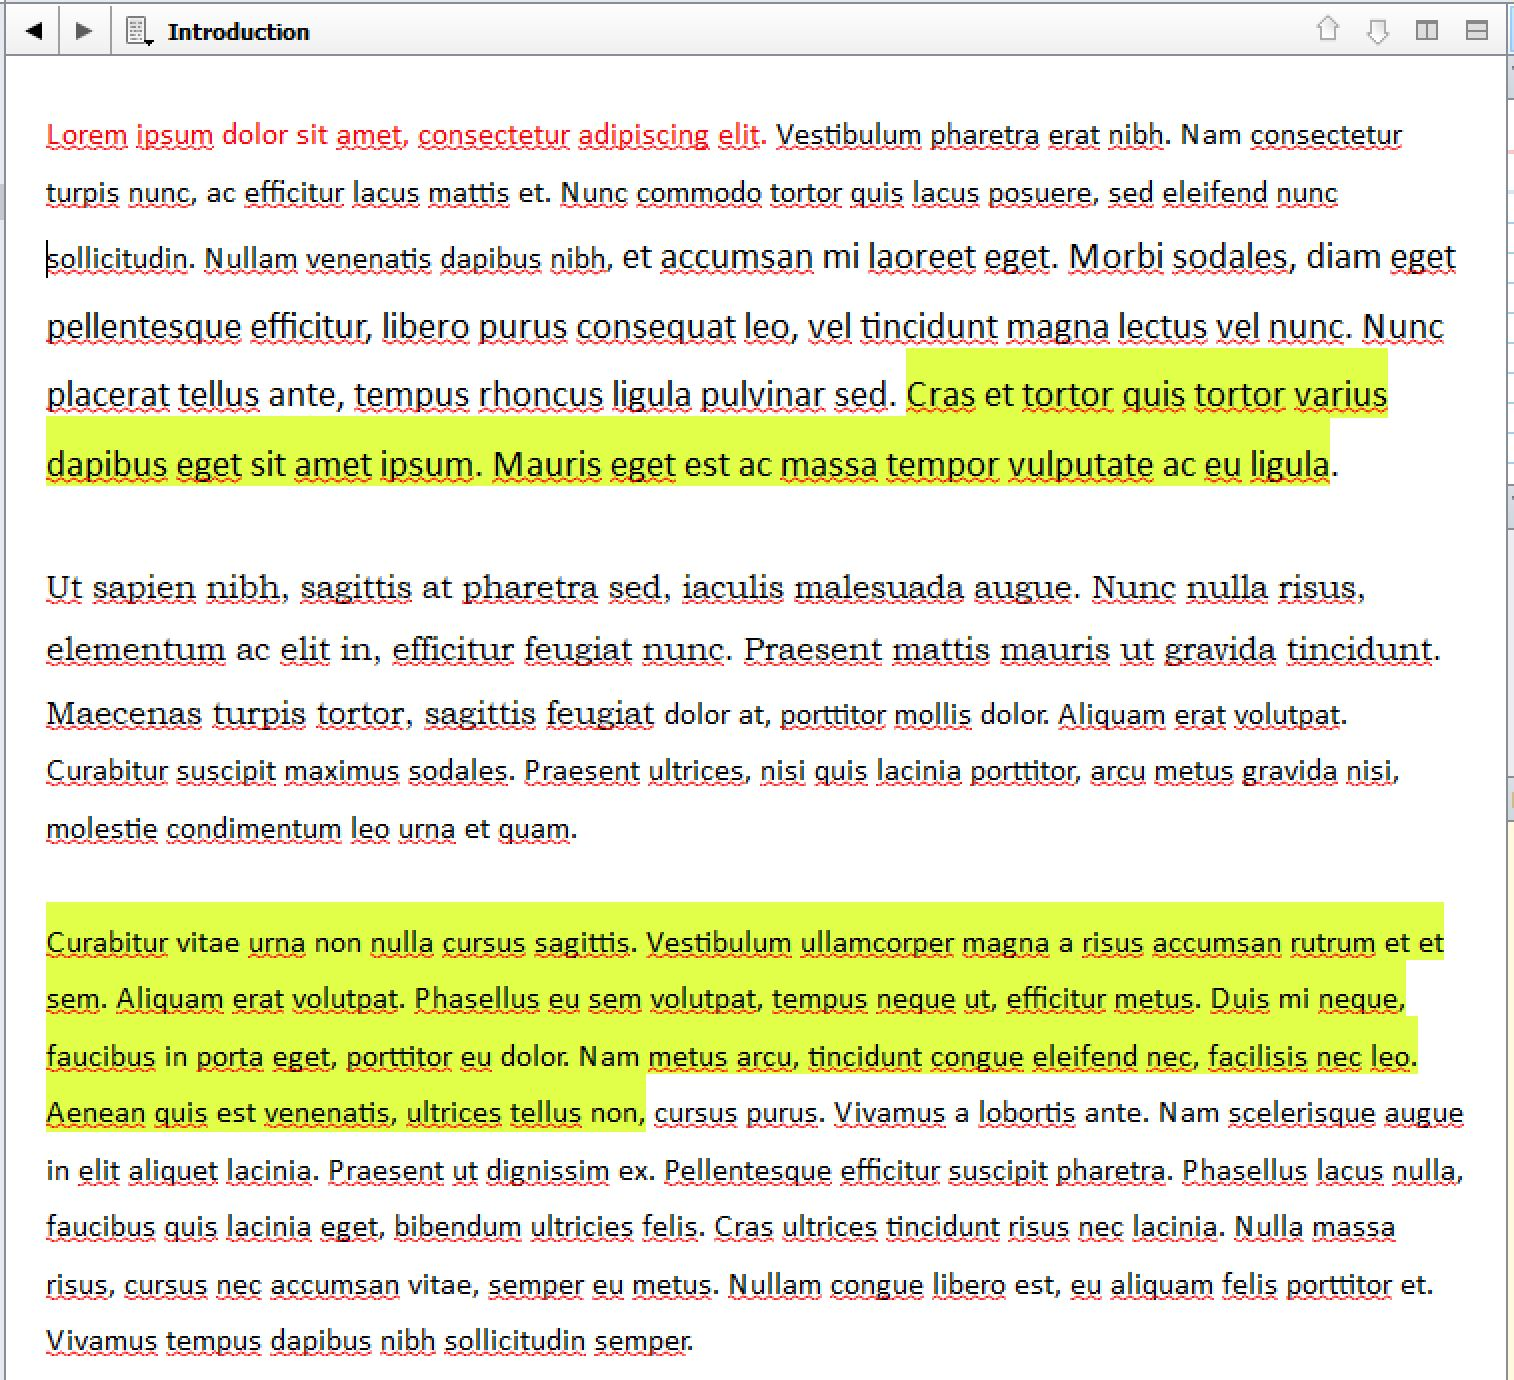
\includegraphics[width=4cm,keepaspectratio]{Images/ScrivMessyText.JPG}
    
      
\columnbreak %Column break point
into this:
 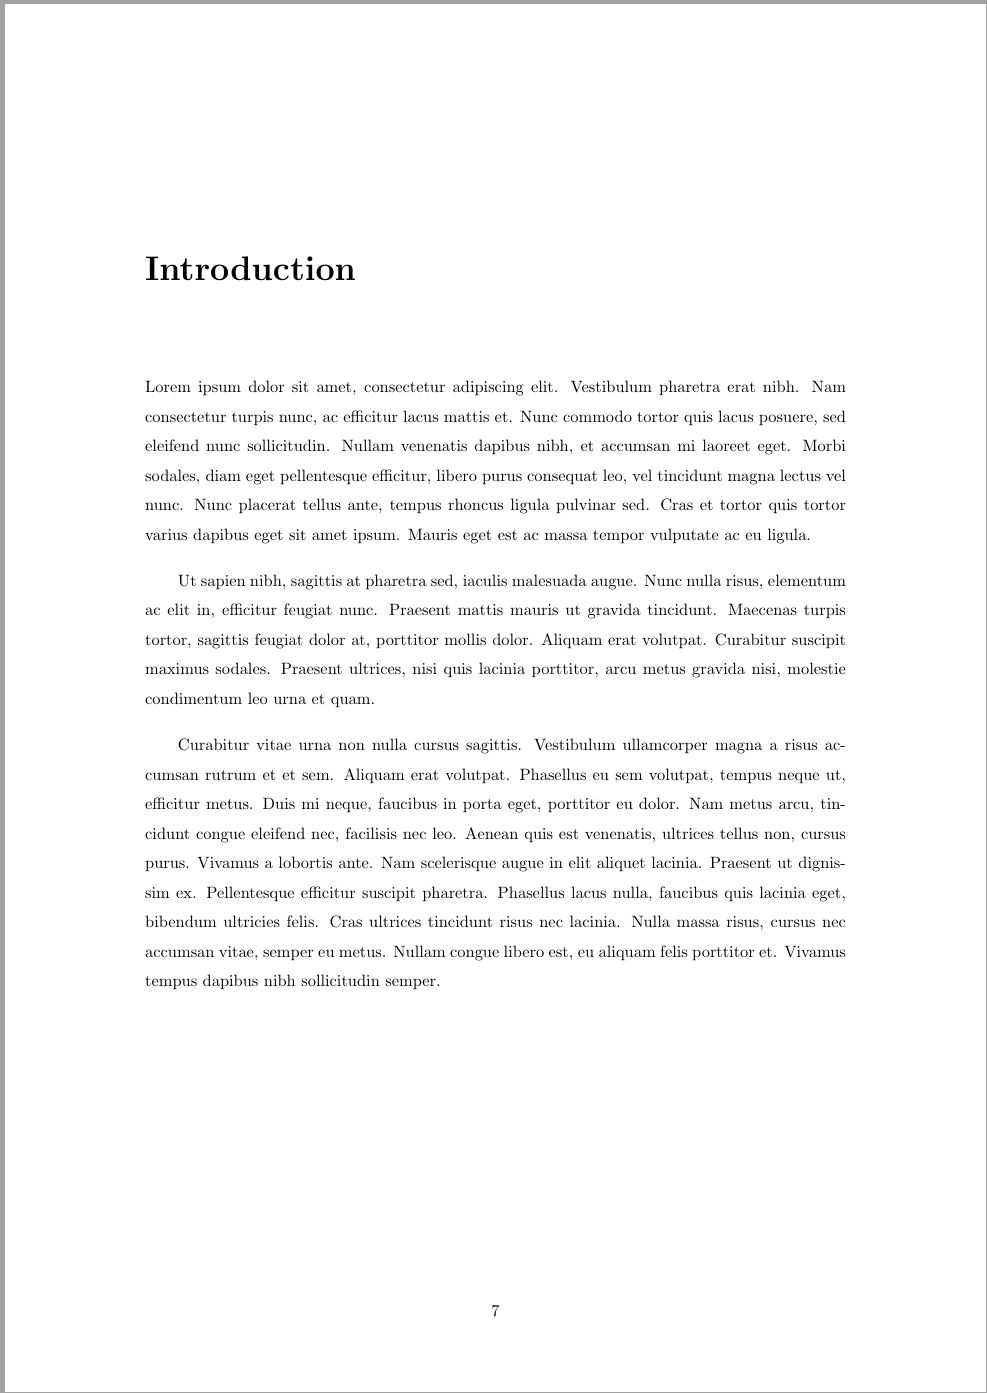
\includegraphics[width=4cm,keepaspectratio]{Images/TexLiveText.JPG}

  \end{multicols*}

  
\end{frame}

%%%%%%%%%%%%%%%%%%%%%%%%%%%%%%%%%%%%%%%%%%%%%%%%%%%%%%%%%%%%%%%%%%%%%%%%%%
\mysection{radar}
%%%%%%%%%%%%%%%%%%%%%%%%%%%%%%%%%%%%%%%%%%%%%%%%%%%%%%%%%%%%%%%%%%%%%%%%%%
\begin{frame}\label{\secvariable}
    \textbf{Scrivener}
    
    Scrivener is available from 
    
    \url{www.literatureandlatte.com}
    
    It is free to download and trial for 30 non-consecutive days. 
    
      \vspace{12pt}
    \textbf{TexLive}  
	
	TexLive is free and is available from \url{www.tug.org/texlive/}
	
	There is also ample online support for tex language
	
	\vspace{12pt}
	
	\textbf{My GitHub Repository}
	
	You can find my GitHub Repository at
	
\url{https://github.com/MQ-FOAR705/SGoldie_ScrivToTexThesis}

This repository contains the template file and compile settings for Scrivener. The instructions explain how to incorporate these with Scrivener, and then use that to export a file to TexLive or Overleaf.
	  
    
  
\end{frame}

%%%%%%%%%%%%%%%%%%%%%%%%%%%%%%%%%%%%%%%%%%%%%%%%%%%%%%%%%%%%%%%%%%%%%%%%%%
\mysection{line}
%%%%%%%%%%%%%%%%%%%%%%%%%%%%%%%%%%%%%%%%%%%%%%%%%%%%%%%%%%%%%%%%%%%%%%%%%%
\begin{frame}\label{\secvariable}
\begin{center}
  \vspace{-0.5cm}
  %http://lorempixel.com/1200/800/cats/Figure4/
 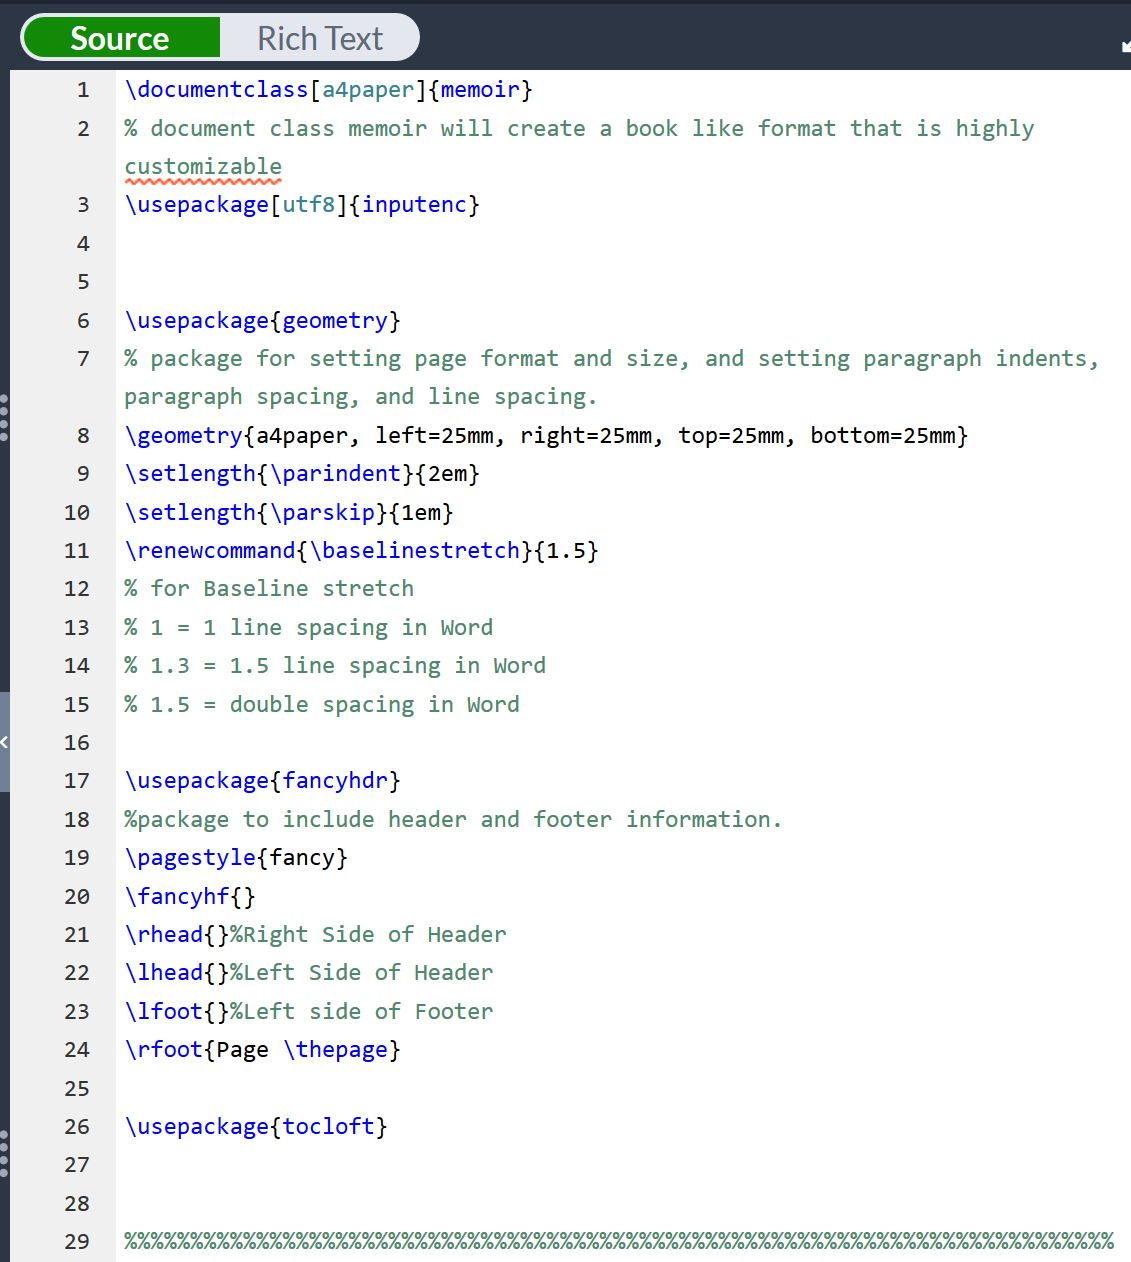
\includegraphics[height=0.65\textheight,keepaspectratio]{Images/OverleafCode.JPG}
\end{center}
  \vspace{-0.5cm}
  
  Pictured is the preamble that I have saved as part of the templates included with my project. 
  
  This LaTeX code, along with some that gets added at the end of the compiled file from Scrivener, set up the formatting guidelines for the document.

  
\end{frame}

%%%%%%%%%%%%%%%%%%%%%%%%%%%%%%%%%%%%%%%%%%%%%%%%%%%%%%%%%%%%%%%%%%%%%%%%%%
\mysection{major}
%%%%%%%%%%%%%%%%%%%%%%%%%%%%%%%%%%%%%%%%%%%%%%%%%%%%%%%%%%%%%%%%%%%%%%%%%%
\begin{frame}\label{\secvariable} %%Eine Folie
\begin{center}
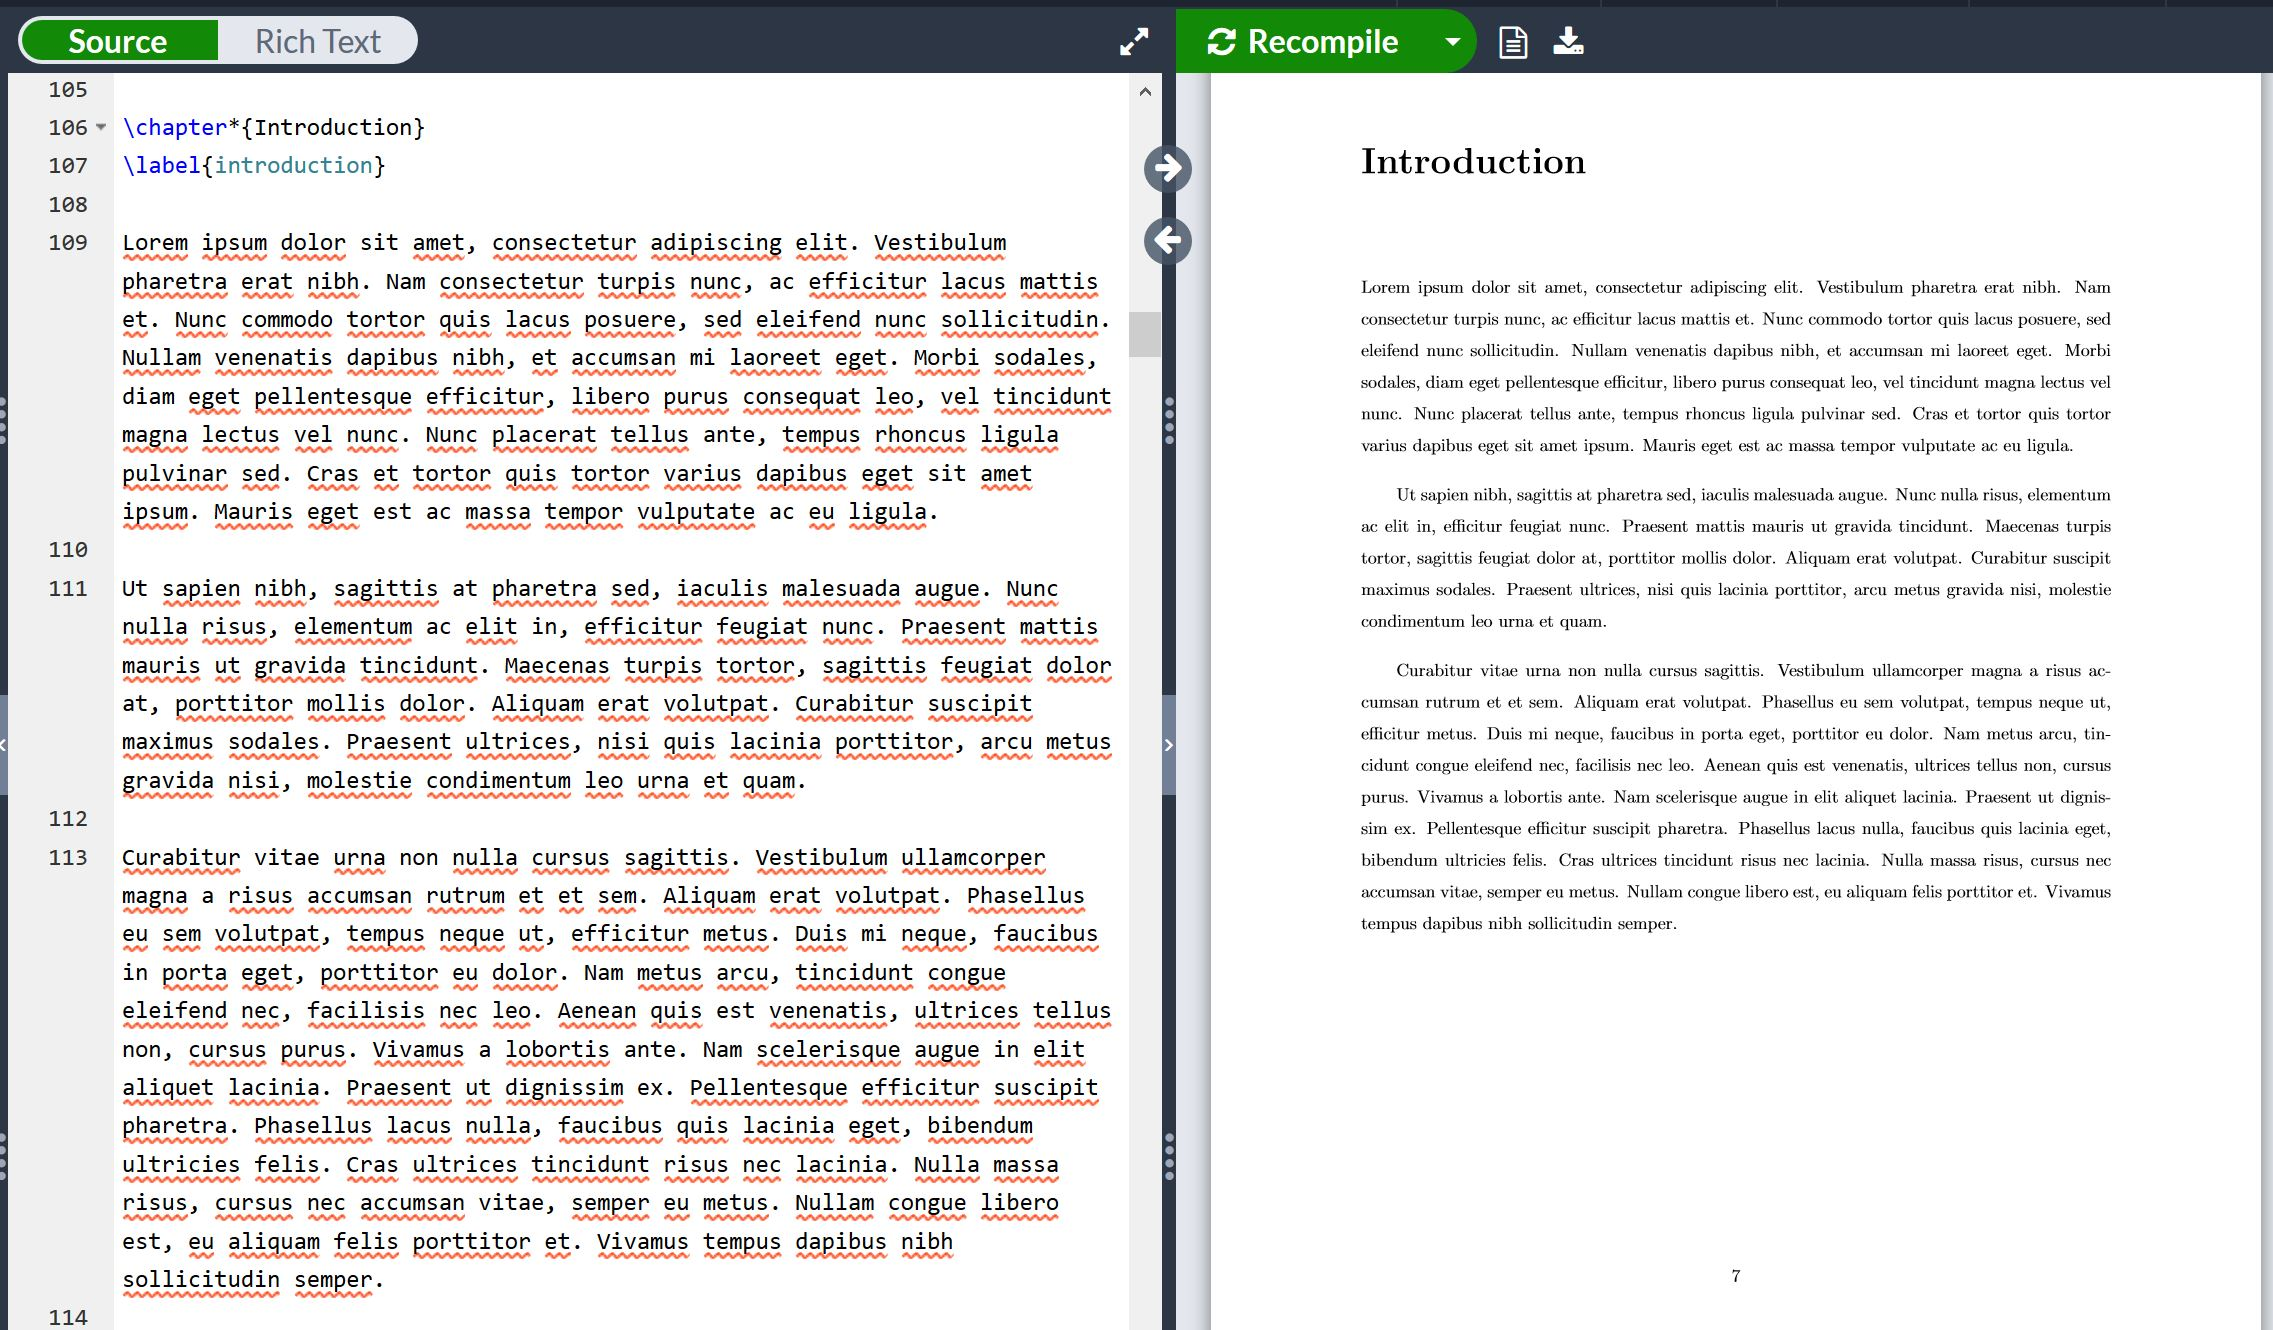
\includegraphics[width=1\textwidth,height=0.6\textheight,keepaspectratio]{Images/OverleafText.JPG}
\end{center}

    \parbox{\linewidth}{
\textbf{Overleaf} is an online alternative to TexLive, that as Macquarie students and staff, we have access to. 
It is convenient to be able to work on projects from any device, but naturally it cannot be accessed without internet.

Pictured is the way you can compose using LaTeX in Overleaf. It is a good way to learn LaTeX as it can compile anytime, and you can troubleshoot issues as you go. 
}
\end{frame}

%%%%%%%%%%%%%%%%%%%%%%%%%%%%%%%%%%%%%%%%%%%%%%%%%%%%%%%%%%%%%%%%%%%%%%%%%%
\mysection{slab}
%%%%%%%%%%%%%%%%%%%%%%%%%%%%%%%%%%%%%%%%%%%%%%%%%%%%%%%%%%%%%%%%%%%%%%%%%%
\begin{frame}\label{\secvariable}

\begin{center}

\includegraphics[width=1\textwidth,height=0.5\textheight,keepaspectratio]{Images/OtherUsesScriv1.JPG}
\hspace{20pt}
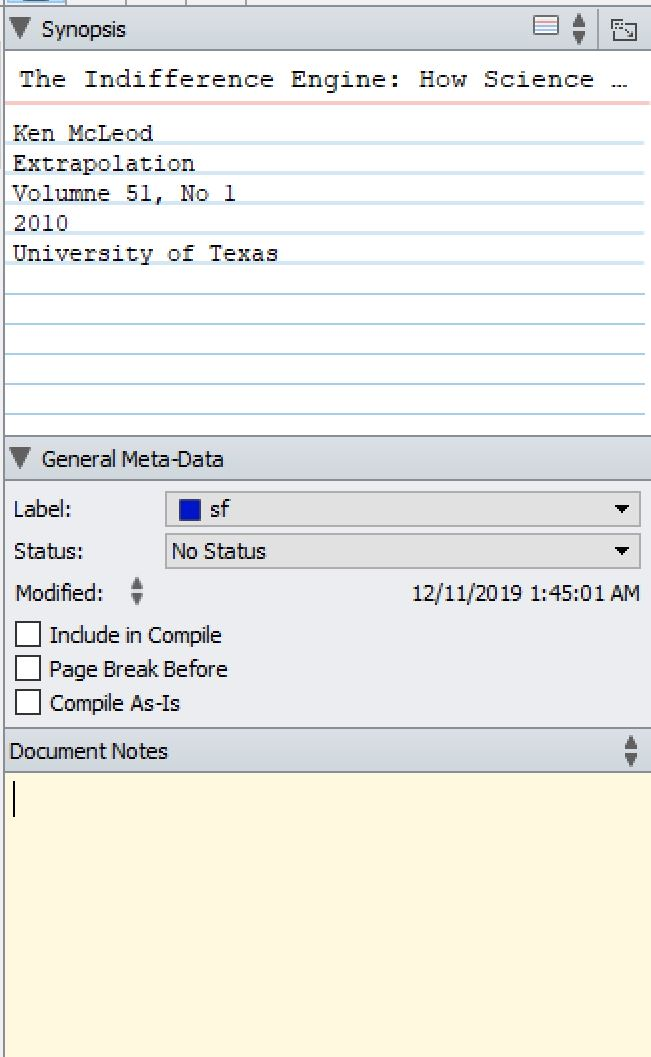
\includegraphics[width=1\textwidth,height=0.5\textheight,keepaspectratio]{Images/OtherUsesScriv2.JPG}
\end{center}
    
    Scrivener is highly useful as a composition tool. It allows for note taking, stores and views PDF document. Each file, and folder, have document note sections, and a simulation of an index card - A perfect place to hold on to source information!
    
\end{frame}


\end{document}
